\chapter{Scaling Difficulties with samtools merge}
\label{app:merge-leak}

\section{Memory Leak}
\ifpdf
    \graphicspath{{Chapter5/Figs/Raster/}{Chapter5/Figs/PDF/}{Chapter5/Figs/}}
\else
    \graphicspath{{Chapter5/Figs/Vector/}{Chapter5/Figs/}}
\fi

By default the \textbf{LSF} job scheduler at the Sanger Institute will issue
100MB to any submitted job. Given both the number of input files and their total
size it was anticipated that this merge job would require more memory. At the
very least an estimated 35kB for a 64-bit pointer to each input file and
approximately 150MB to house a 32kB buffer to read data from each file also. Yet
executing the job with 500MB of memory caused the scheduler to forceably
terminate the process for exceeding the maximum allocated memory limit.

Assuming that the intermediate structures for storing and sorting the input data
must have been greater than expected, the job's memory limit was generously
increased with the syntax previously demonstrated by
Listing~\ref{list:lsf-memory} only to meet the same fate, even when reserving
16GB of memory. Even considering the thousands of input files this is an absurd
amount of memory, I'd discovered a memory leak, a leak that appeared to
drastically increase in severity in proportion to the number of input files.

Once reported, the leak was fixed by the author; several large variables
constructed when translating the input format were not freed when no longer
needed. Despite this, during execution of the \textbf{samtools} test suite, a
series of leaks were still being reported.


\section{Memory Leak in Test Harnesses}
%TODO Cite valgrind

Wanting to brush up on finding memory leaks with \textbf{valgrind}, I
volunteered to find and patch the remaining reported leaks. The results of this
investigation are detailed in Appendix~\ref{app:test-leaks}.

...getline
...regcomp...


% https://github.com/samtools/samtools/pull/200
% http://valgrind.org/docs/manual/cl-manual.html

\begin{listing}[H]
    \caption[valgrind-regex]{: Example of \textbf{valgrind} locating a memory
        leak in one of the \textbf{samtools} test harnesses following the failure
        to release memory allocated to a compiled regular expression}
    \label{list:valgrind-regex}
    \begin{minted}[mathescape,
                %linenos,
                gobble=8,
                fontsize=\footnotesize,
                frame=lines,
                framesep=2mm]{bash}
        ==30464== 416 bytes in 1 blocks are indirectly lost in loss record 85 of 103
        ==30464==    at 0x4A082F7: realloc (in /usr/lib64/valgrind/vgpreload_memcheck-amd64-linux.so)
        ==30464==    by 0x3FBCCCA725: duplicate_node (in /usr/lib64/libc-2.17.so)
        ==30464==    by 0x3FBCCD3ADA: duplicate_node_closure (in /usr/lib64/libc-2.17.so)
        ==30464==    by 0x3FBCCD415A: calc_eclosure_iter (in /usr/lib64/libc-2.17.so)
        ==30464==    by 0x3FBCCD79F6: re_compile_internal (in /usr/lib64/libc-2.17.so)
        ==30464==    at 0x4A08121: calloc (in /usr/lib64/valgrind/vgpreload_memcheck-amd64-linux.so)
        ==30464==    by 0x3FBCCCCD88: create_cd_newstate (in /usr/lib64/libc-2.17.so)
        ==30464==    by 0x3FBCCCD506: re_acquire_state_context.constprop.41 (in /usr/lib64/libc-2.17.so)
        ==30464==    by 0x3FBCC2132E: build_trtable (in /usr/lib64/libc-2.17.so)
        ==30464==    by 0x3FBCCD3792: re_search_internal (in /usr/lib64/libc-2.17.so)
        ==30464==    by 0x3FBCCD8E94: regexec@@GLIBC_2.3.4 (in /usr/lib64/libc-2.17.so)
        ==30464==    by 0x40C6FA: check_test_2 (test_trans_tbl_init.c:124)
        ==30464==    by 0x402CC4: main (test_trans_tbl_init.c:348)
    \end{minted}
\end{listing}

...following this, further \textbf{samtools merge} jobs were submitted only to
also be repeatedly terminated by the LSF scheduler , this time for exceeding the
maximum execution time limit for the queue...

\section{Poor Time Performance}
...submitting the same job to the "long" (48hr) and "basement" (essentially
unlimited) queues, it is clear that the job is taking an extraordinary length of
time to complete...

...during this time I took the opportunity to patch various memory leaks in the
test harnesses of both merge and split...

% http://kcachegrind.sourceforge.net/html/Home.html
% http://www.zlib.net/
valgrind, the tool I used to track down memory leaks in the test harnesses of
both samtools merge and samtools split actually consists of more than just
memcheck.

callgrind is a profiling tool that keeps track of a program’s call stack
history, a handy feature built in to some development environments such as
QtCreator.

Having constructed a modest test set of files to merge, I called samtools merge
from the command line, attaching callgrind and later imported the resulting
text file to QtCreator’s profiling tool to interpret the results (I usually use
KCacheGrind for this but I’ve been investigating QtCreator’s feature set for
reasons unrelated to this project), the result is immediately obvious -
millions of calls to functions in zlib; a free compression library.

% https://github.com/samtools/htslib/blob/develop/bgzf.c#L220
Further investigations using the QtCreator Analyze interface revealed that
these calls all boiled down to one line called not during the process of
deflating the input files (as I had expected) but actually during the
compression of the output!

\begin{figure}[htbp!]
    \centering
    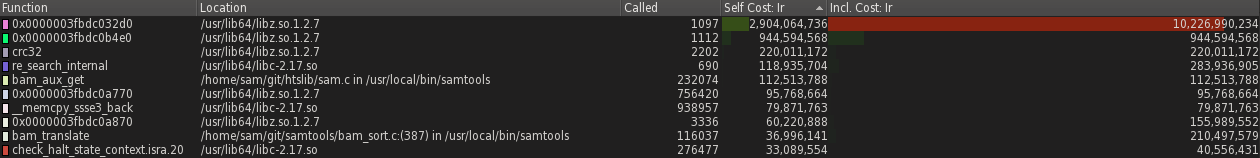
\includegraphics[width=1.0\textwidth]{callgrind_compressoutput_default}
    \caption[callgrind-default]{callgrind output following merge with default
    output compression}
    \label{fig:callgrind-default}
\end{figure}

\begin{figure}[htbp!]
    \centering
    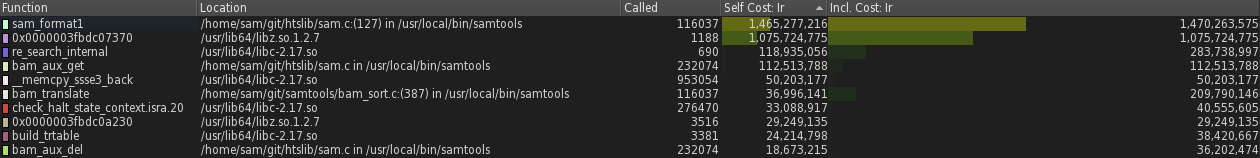
\includegraphics[width=1.0\textwidth]{callgrind_uncompressoutput}
    \caption[callgrind-uncompressed]{callgrind output following merge with
    uncompressed output}
    \label{fig:callgrind-uncompressed}
\end{figure}

% http://www.zlib.net/feldspar.html
Looking at a brief explanation of the deflate algorithm, it seems reasonable to
conclude the computational cost is rather asymmetric between compressing and
uncompressing - in that the effort is locating blocks to compress and in
comparison uncompressing is a reversible function on the known blocks.

Indeed, samtools merge specifies a -u option for uncompressed output and the
callgrind output (second image) indicates significantly less calls to zlib
functionality.

It remains to be seen whether this option will cut down the time needed for the
large merge job, perhaps this is merely a red herring and we’re yet to discover
the true speed trouble. In the meantime let’s see if sending this job to the
farm will work.


\section{The Red Herring}

% http://www.cs.utah.edu/dept/old/texinfo/as/gprof.html
... might be interesting to use gprof which is more
geared towards finding functions that spend all your execution time as opposed
to callgrind which I believe counts CPU instructions.

% http://paste.chippy.ch/woj.md
% https://github.com/samtools/htslib/blob/develop/sam.c#L1031
After re-compiling htslib and samtools with the -pg flag to enable such
profiling and executing the same previous merge command on the modest test set,
the output as parsed by gprof seems to indicate that the trouble lies with
bam\_aux\_get in htslib, with almost 50\% of the execution time being spent in
this particular function.

\begin{minted}[mathescape,
            %linenos,
            numbersep=5pt,
            %gobble=4,
            frame=lines,
            framesep=2mm]{c++}
    uint8_t *bam_aux_get(const bam1_t *b, const char tag[2])
    {
        uint8_t *s;
        int y = tag[0]<<8 | tag[1];
        s = bam_get_aux(b);
        while (s < b->data + b->l_data) {
            int x = (int)s[0]<<8 | s[1];
            s += 2;
            if (x == y) return s;
            s = skip_aux(s);
        }
        return 0;
    }
\end{minted}


% http://samtools.github.io/hts-specs/SAMv1.pdf
At a glance it seems that bam\_aux\_get receives a pointer to a BAM record and a
“tag”, an array of two characters representing an optional field as defined in
Section 1.5 of the SAM file spec.

The function then appears to fetch all these auxiliary tags and iterates over
each, comparing a transformation of that tag (x) to a pre-computed
transformation on the input tag (y).

% https://github.com/samtools/samtools/blob/2917ccdf34cd81b1327532b2db6e522fe871f054/bam_sort.c#L469
% https://github.com/samtools/samtools/blob/2917ccdf34cd81b1327532b2db6e522fe871f054/bam_sort.c#L484
% https://github.com/samtools/samtools/blob/2917ccdf34cd81b1327532b2db6e522fe871f054/bam_sort.c#L697
This would of course be inherently slow for files with many such tags;
especially given that the function is called twice for potentially each line in
a BAM file.


\section{The Plot Thickens}

% https://github.com/samtools/samtools/blob/2917ccdf34cd81b1327532b2db6e522fe871f054/bam_sort.c#L207
...as we increase the number of input files, the time taken to
read them in becomes non-linearly slower. Currently my money is on the seemingly
inefficient trans\_tbl\_init that appears to be called for each file, with the
current table of all previous files as an input...
